% LaTeX template for SAS Deliverables and Reports
% Based on the template prepared by Luigi Freda and Alessandro De Luca (UOR)
% November 2008
% edited by Raul Sena Ferreira (LAAS)
% November 2019

\documentclass[11pt,a4paper]{article}

\usepackage{sas} % INCLUDED in the directory
\usepackage{graphicx}
%\usepackage[none]{hyphenat}
%\usepackage{longtable}
\usepackage[english]{babel}
\usepackage{fancyhdr}
\usepackage{array}
\usepackage{color}
\usepackage{colortbl} %required for color tables in report cover page
\usepackage{sectsty}
\usepackage{pdflscape}
\usepackage{multirow}
\usepackage[utf8]{inputenc}
\usepackage{amsfonts, amsmath, amsthm}
\usepackage{threeparttable}
\usepackage{xargs}
\usepackage{microtype}
\usepackage{booktabs}
\usepackage{comment}
\usepackage{dblfloatfix}
\usepackage{adjustbox}
\usepackage{algpseudocode,algorithm}
\usepackage{algorithmicx}
\usepackage{pgfplots}
\usepackage{caption}
\usepackage{subcaption}
\usepackage{float}
\usepackage{array}
\pgfplotsset{compat=newest}

%%%%%%%%%%%%%%%%%%%%%%%%%%%%%%%%%%%
\begin{document}
\color{black} % set default text color
\sectionfont{\centering}
\pdfinfo{
/Title (Your title)
/Author (author 1, author 2...)
}
%%%%%%%%%%%%%%%%%%%%%%%%%%%%%%%%%%%%             ********     COVER PAGE    **********
\MakeCoverPage
%%%%%%%%%%%%%%%%%%%%%%%%%%%%%%%%%%%%            ******   EXECUTIVE SUMMARY    ******
\section*{Summary}
%\begin{center}
Here you can put the summary of your report
%\end{center}
\thispagestyle{fancy}
\clearpage
%%%%%%%%%%%%%%%%%%%%%%%%%%%%%%%%%%%           ********   TABLE OF CONTENTS    ********
\phantomsection
\renewcommand{\contentsname}{\centering {\bf TABLE OF CONTENTS}}
%{\em \tableofcontents} %italic style
{\bf \tableofcontents}      %boldface style
%\tableofcontents           %roman style
%\thispagestyle{fancy}
\clearpage
%%%%%%%%%%%%%%%%%%%%%%%%%%%%%%%%%%%             ******        REPORT          ********
\pagestyle{fancy}
\section{Introduction}
Just an example of structure and file organization. You can put the name of the Sections as you want.
This is the way that you can make a citation~\cite{ferreira2019amanda}.
For changing the cover page go to sas.sty file and look for the comment "Cover Page".
\section{Section 2}
You can \textbf{write bold texts} and lists:
\begin{itemize}
    \item Item 1.
    \item Item 2.
    \item Item 3.
\end{itemize}
\section{Section 3}
Below you can find an example of a Table \ref{table:MLlandscape} and how you can change the orientation of a page using "landscape" tag:

\begin{landscape}

\begin{table}[!htb]
\centering
\caption{Caption.}
%\resizebox{\linewidth}{!}
\label{table:MLlandscape}
\end{table}

\end{landscape}

\section{Section 4}
Below an example of sub-section

\subsection{Monitoring ML components as a black box} 
Below an example of Figure\ref{fig_example}.

\begin{figure}[htb]
\centering
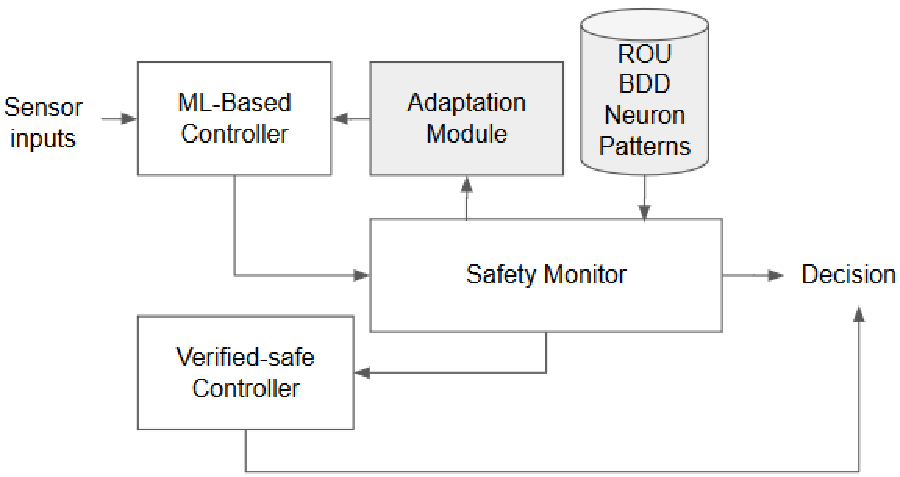
\includegraphics[width=.52\linewidth]{img/proposal.pdf}
\caption{Figure caption.} \label{fig_example}
\end{figure}
\section{Section 5}
The bibliography can be added in the Bibliography.bib file

%%%%%%%%%%%%%%%%%%%%%%%%%%%%%%%%           ******      BIBLIOGRAPHY      ********
\addcontentsline{toc}{section}{References}
\bibliographystyle{amsplain}
\bibliography{Bibliography}

\end{document}